\begin{figure}[] \centering
	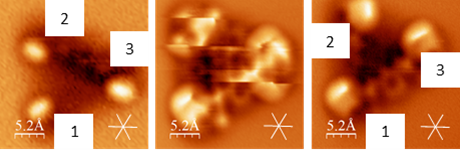
\includegraphics[width=0.7\textwidth]{./images/hbbnc-ag-111-leg-flip}
	\caption{Conformational change of a monomer after several scans with the AFM. First the molecule starts with an orientation of the legs in 1: clockwise, 2: counterclockwise, 3: clockwise. After several scans in close proximity legs at positions 2 and 3 flip around and change their orientation to 1: clockwise, 2: clockwise, 3: counterclockwise. This results in a changed adsorption geometry. First the upper right edge is lifted from the substrate, while after the leg rearrangement the lower right edge is lifted from the surface. This is caused by the lower lying dimethyl groups lifting the phenyl ring and the molecules edge.}
	\label{fig:HBBNC-nc-AFM-legs-change}
\end{figure}

\begin{figure}[] \centering
	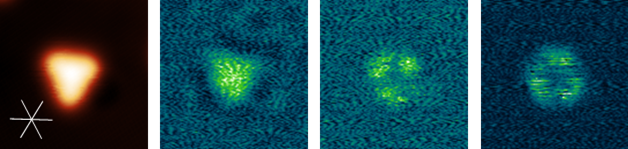
\includegraphics[width=0.7\textwidth]{./images/hbbnc-maps}
	\caption{STM Topography image and dI/dV maps for chosen energies. Choosing the spectroscopy energy to match one of the spectral maxima of the line spectra reveals the spatial distribution of electronic states as shown by the maps. While at 650 meV only the core contributes to the DOS, energies of 1200 meV and 1600 meV are located on the leg and edge positions respectively.}
	\label{fig:HBBNC-Ag111-dIdV-maps}
\end{figure}

\begin{figure}[] \centering
	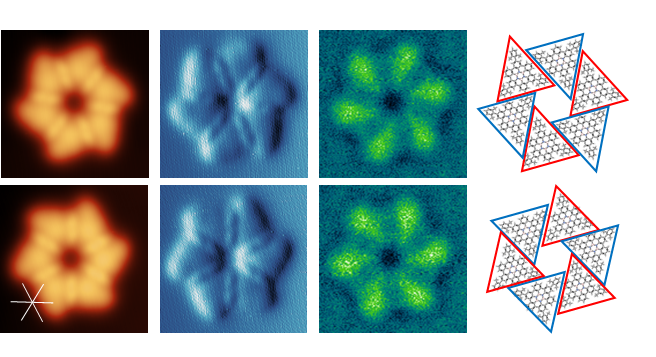
\includegraphics[width=0.7\textwidth]{./images/hbbnc-maps2}
	\caption{Comparison of two hexamers (chiral twins). While in STM the most apparent change is the orientation of the molecules within the hexamer and the resulting change in the protrusion between them, dI/dV maps (600 meV) clearly highlight the turn direction within the hexamer.}
	\label{}
\end{figure}

\begin{figure}[] \centering
	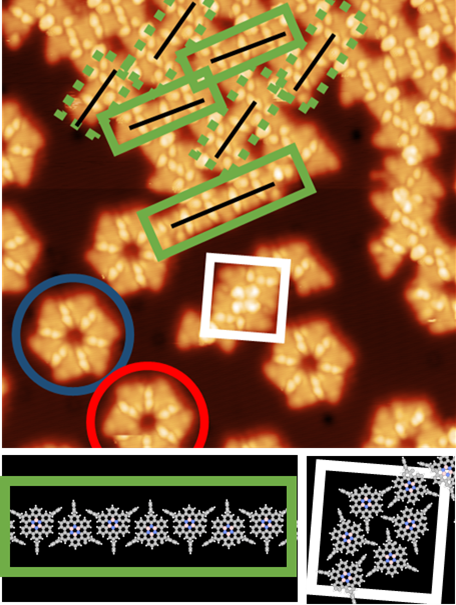
\includegraphics[width=0.7\textwidth]{./images/hbbnc-ag-111-rt-med-coverage-3}
	\caption{Medium coverage adsorption of HBBNC at RT on Ag(111). While the chiral assemblies are still present (blue/red circles), additional binding motifs like chains (green boxes) occur. Square  binding motifs are less frequent (white box). Imaging parameter: \SI{22.1}{\nano \meter}, \SI{2}{\volt}, \SI{0.4}{\nano \ampere}, Color scale: \SIrange{0}{400}{\pico \meter}.}
	\label{fig:HBBNC-medium-coverage-different-motifs}
\end{figure}

\begin{figure}[] \centering
	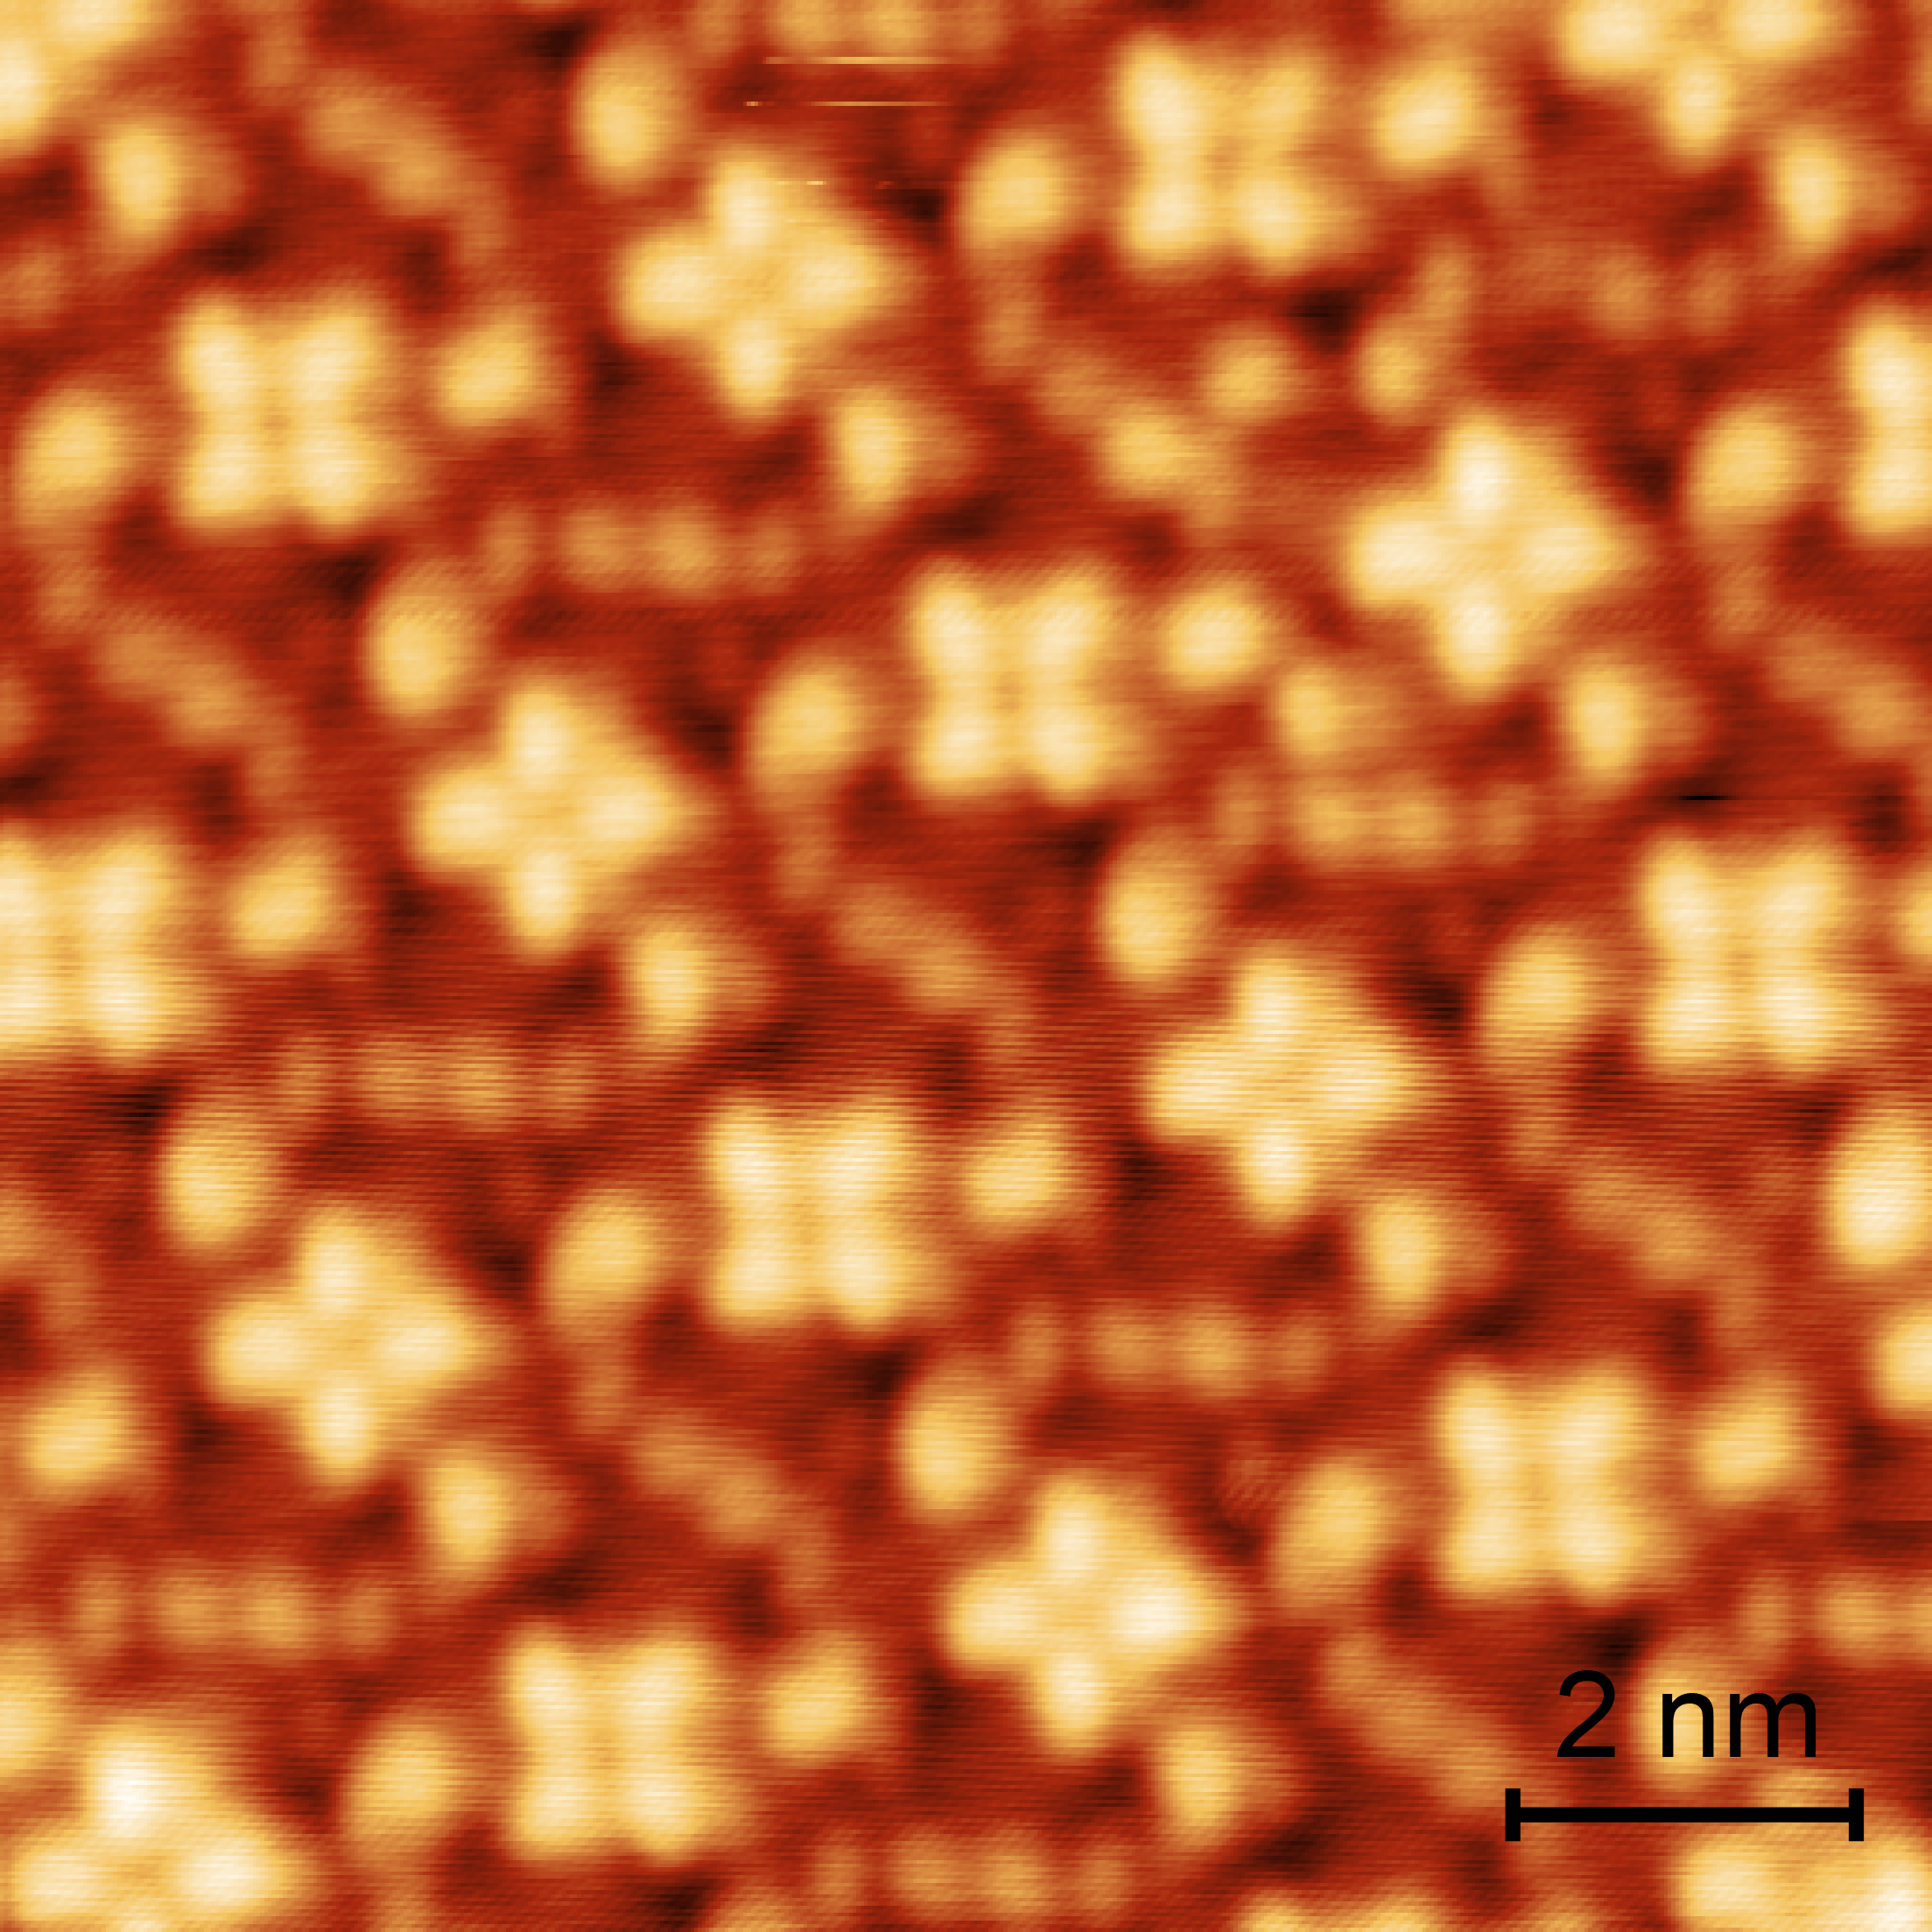
\includegraphics[width=0.7\textwidth]{./images/A180515-095412}
	\caption{STM topography image for high coverage adsorption of HBBNC at RT on Ag(111). The dominating pattern is the clover-leaf resembling the one observed for medium coverage. It is present here in two different orientations and distributed such that neighboring squares do not show the same orientation. Two squares with the same orientation are separated by lines made up of four bright spots aligned parallel to the square edge and diagonal. Squares with different rotations show a single protrusion with larger apparent height. Imaging parameter: \SI{11.07}{\nano \meter}, \SI{-250}{\milli \volt}, \SI{0.2}{\nano \ampere}.}
	\label{fig:HBBNC-high-coverage}
\end{figure}

\begin{figure}[] \centering
	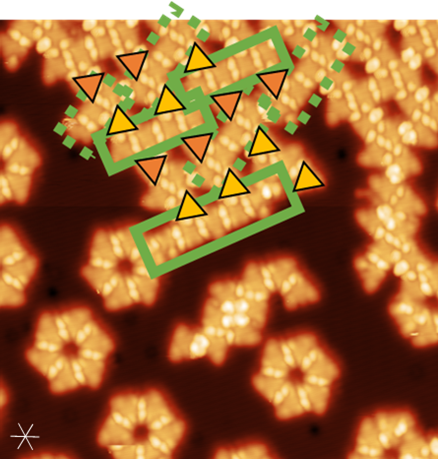
\includegraphics[width=0.7\textwidth]{./images/hbbnc-ag-111-rt-med-coverage-spacer-mol}
	\caption{Rows are separated by two sets of spacer molecules (orange/yellow). 
		\textcolor{red}{\textbf{What is their position in the unit cell? Rotation? Separation to all the other molecules?}}
	}
	\label{}
\end{figure}

